\section{Definición de la tarea} \label{tarea}

En la siguiente tarea se solicita crear tres peticiones o query a un servidor desde una interfáz web. Estas peticiones deben ser de gran esfuerzo, es decir, se debe procesar una gran cantidad de datos desde la base de datos.\\

Posteriormente realizadas estas query se deben realizar 5 iteraciones para omptimizar estas solicitudes. Estas iteraciones buscan reducir los tiempos de espera del usuario que solicita la gran cantidad de datos a la base de datos.\\

Finalmente realizadas las iteraciones que buscan otpimizar las solicitudes. Se debe realizar una pruebas de carga con la herramienta Jmeter. Estas pruebas buscan estudiar el comportamiento de estas mismas consultas optimizadas pero suponiendo que varios usuarios accederán a ellas en un tiempo simultaneo. Cabe mencionar que las pruebas se deben realizar en un entorno "limpio", es decir, suponer que el dispositivo del usuario no se ve afectado por otros programas o por otros problemas de rendimiento. \\

\section{Consultas Básicas a la base de datos mediante una interfáz web}

En un comienzo se realizó una interfaz web simple, la cual cuenta con 3 botones, en donde cada botón al presionarlo genera una consulta a la base de datos \textbf{"employees"} como se muestra en las siguientes figuras \ref{Figura2}, \ref{Figura4}, \ref{Figura6}. \\ 
Cabe mencionar que cada una de estas query se realiza de forma inmediata luego de presionar el botón, y no de la forma en que trabaja CodeIgniter ( Modelo-Vistra-Controlador). \\
Además previo a realizar cada consulta se realizan las siguientes acciones: 

\begin{figure}[htb]
	\label{Figura0}
	\begin{center}
		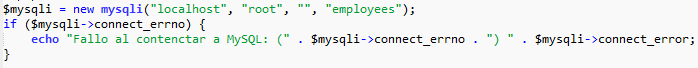
\includegraphics[scale=0.5]{imagenes/acciones.png}
	\end{center}
	\caption{Esta figura muestra las acciones a realizar previo a llevar a cabo una query la cual se repite para las 3 consulas.}
\end{figure}

\begin{figure}[htb]
	\label{Figura}
	\begin{center}
		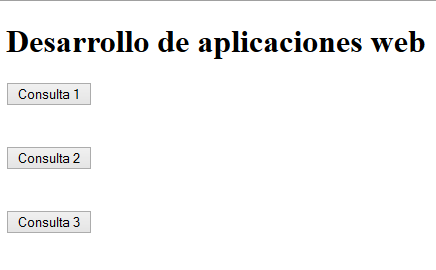
\includegraphics[scale=0.5]{imagenes/inicio.png}
	\end{center}
	\caption{Figura de la interfáz de inicio de la página web de consultas.}
\end{figure}

\subsubsection{Consulta 1}

El usuario al presionar el botón "Consulta 1" se realiza la siguiente query:

\begin{figure}[htb]
	\label{Figura2}
	\begin{center}
		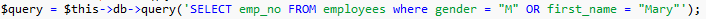
\includegraphics[scale=0.7]{imagenes/query1.png}
	\end{center}
\end{figure}

Esta consulta solicita a la base de datos el "emp\_no" o número de empleado, de los cuales su genero es "M" o masculino, O también el número de empleados cuyo nombre sea "Mary".

Los resultados entregados por el servidor son los que se muestran en la figura \ref{Figura3}:

\begin{figure}[htb]
	\label{Figura3}
	\begin{center}
		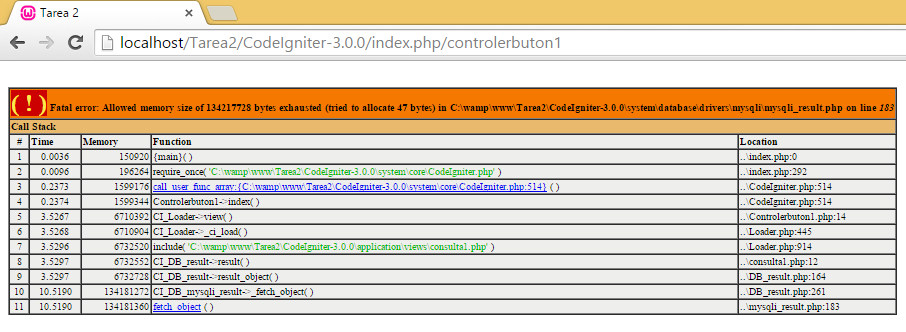
\includegraphics[scale=0.7]{imagenes/resultado1.png}
		\caption{Figura que muestra el resultado obtenido desde el servidor, en donde se muestran algunos números de empleados.}
	\end{center}
\end{figure}

\subsubsection{Consulta 2}

El usuario al presionar el botón "Consulta 2" se realiza la siguiente query:

\begin{figure}[htb]
	\label{Figura4}
	\begin{center}
		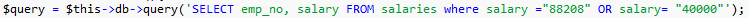
\includegraphics[scale=0.7]{imagenes/query2.png}
	\end{center}
\end{figure}

Esta consulta solicita a la base de datos el "emp\_no" o número de empleado, de los cuales su genero es "M" o masculino, O también el número de empleados cuyo nombre sea "Mary".

Los resultados entregados por el servidor son los que se muestran en la figura \ref{Figura5}:

\begin{figure}[htb]
	\label{Figura5}
	\begin{center}
		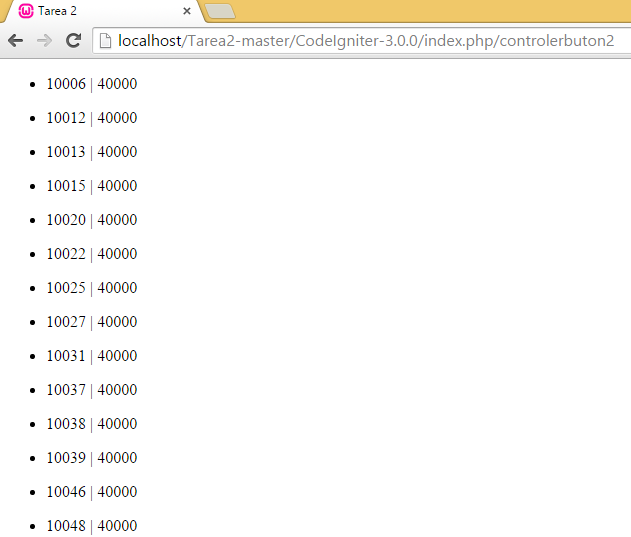
\includegraphics[scale=0.7]{imagenes/resultado2.png}
		\caption{Figura que muestra el resultado obtenido desde el servidor, en donde se muestran algunos números de empleados.}
	\end{center}
\end{figure}

\subsubsection{Consulta 3}

El usuario al presionar el botón "Consulta 3" se realiza la siguiente query:

\begin{figure}[htb]
	\label{Figura6}
	\begin{center}
		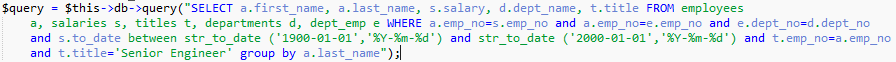
\includegraphics[scale=0.7]{imagenes/query3.png}
	\end{center}
\end{figure}

Esta consulta solicita a la base de datos el "emp\_no" o número de empleado, de los cuales su genero es "M" o masculino, O también el número de empleados cuyo nombre sea "Mary".

Los resultados entregados por el servidor son los que se muestran en la figura \ref{Figura7}:

\begin{figure}[htb]
	\label{Figura7}
	\begin{center}
		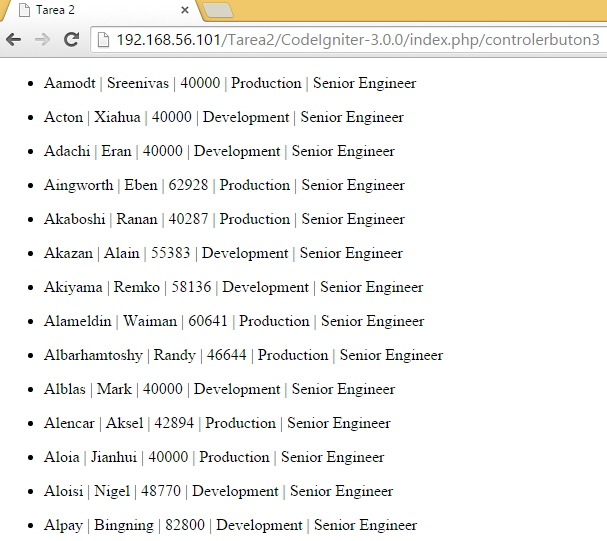
\includegraphics[scale=0.7]{imagenes/resultado3.png}
		\caption{Figura que muestra el resultado obtenido desde el servidor.}
	\end{center}
\end{figure}

\section{Pruebas realizadas a la iteración 0}
 
 En la siguiente sección se muestran los resultados de las pruebas de carga realizadas con la herramienta Jmeter, para realizar estas pruebas se levantó un servidor utilizando Virtual Box con el fin de obtener resultados en un ambiente controlado, libre de otros procesos o programas que puedan interferir en la memoria de nuestro equipo. \cite{jmeter} \\
 
 La maquina virtualizada tiene las siguientes carácteristicas:
 
 \begin{figure}[htb]
 	\label{Figura8}
 	\begin{center}
 		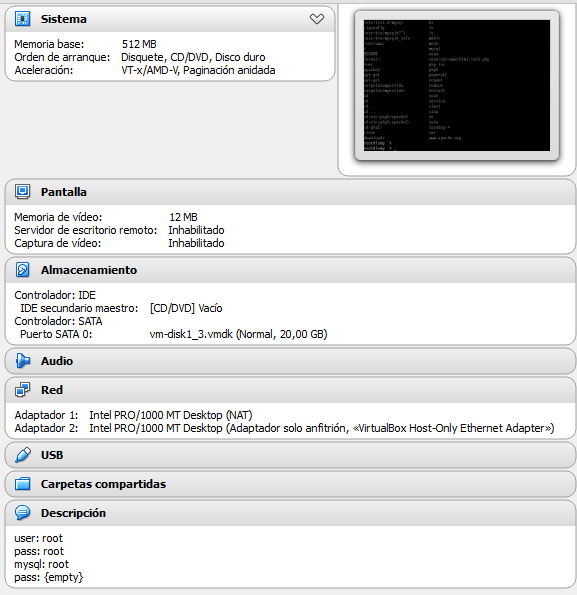
\includegraphics[scale=0.7]{imagenes/sistema.png}
 		\caption{Figura que muestra las carácteristicas de la maquina virtual utilizada.}
 	\end{center}
 \end{figure}
 
Los resultados obtenidos para la consulta 1 fueron los siguientes: 

Los resultados obtenidos para la consulta 2 fueron los siguientes: 

Los resultados obtenidos para la consulta 3 fueron los siguientes: 
 
\section{Iteración 1 ( Mejorando las consultas MySql)} 

Luego de realizar las respectivas pruebas de cargas, se optó por modificar las query MySql, en donde: 


\begin{itemize}
	\item Consulta 1: En la cosnulta 1, se solicita al servidor todos los atributos de la tabla 'employees' ya que se realiza de la forma "SELECT * FROME employees" y donde finalmente se muestra solo "emp\_no" ( Numero de empleado). Por lo cual una mejora a esta query sería solicitar solamente lo que necesitamos, es decir, "emp\_no".\\
	
	\item Consulta 2: En esta consulta se utiliza el operador lógico OR, el cual investigando, se puede mejorar utilizando el operador IN, ell cual entrega un mejor performance al momento de realizar una query.\\
	
	\item Consulta 3: 
\end{itemize}

\section{Pruebas de carga a la iteración 1}

\section{Iteración 2 (Utilizando CodeIgniter)}

Debido a que este Framework ofrece la utilización del Modelo - Vista - Controlador, nos parece pertinente utilizar esta arquitectura, por lo cual se adapta completamente la forma en la que se se escribe el código de este proyecto. \\

La interfáz web sigue siendo la misma, sin embargo, esta interfáz es manjeda por un controlador, el cual se encarga de cargarla.\\

Posteriormente cuando el usuario presiona un botón para llevar a cabo las consultas, es un controlador el encargado de realizar la acción, donde cada botón es manejado independientemente. Posterior a realizar esta acción es el controlador el que solicita al modelo realizar una query al servidor. El modelo realiza la query y envía los datos nuevamente al controlador, para que este se los envíe a la vista para que estos datos puedan ser mostrados al usuario. 

 \begin{figure}[htb]
 	\label{Figura9}
 	\begin{center}
 		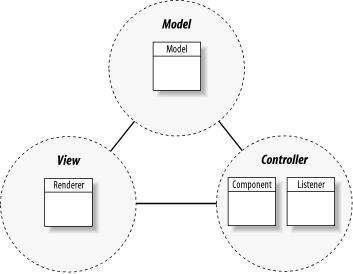
\includegraphics[scale=0.5]{imagenes/mvc.JPG}
 		\caption{Esta imagen ejemplifica como funciona el Modelo - Vista - Controlador.}
 	\end{center}
 \end{figure}
 
 Usando CodeIgniter además nos ahorramos realizar las conexiones a la base de datos, ya que internamente se configura la base de datos que se utilizará. 
 
 \section{Pruebas de carga realizadas a la iteración 2}
 
 \section{Iteración 3 (Utilizando la opción de Cachè en CodeIgniter))}
 
 Como además CodeIgniter ofrece la utilización de Cachè, las consultas obendrá un mejor desempeño, ya que luego de realizar una de las query, los datos estarán "Cacheados" por lo cual, las posteriores consultas deberían resultar ser mas rápidas. 
 
 \section{Pruebas de carga realizadas a la iteración 3}
 
 \section{Iteración 4 (Paginación de los resultados de las query)}  

